\section{Problema 2: Alta Frecuencia}
\subsection{Descripci\'on de la problem\'atica}

Se quiere transmitir informaci\'on secuencialmente mediante un enlace el mayor tiempo posible. Los enlaces tienen asociadas distintas frecuencias, con un costo por minuto y un intervalo de tiempo (sin cortes) en el cual funcionan. Se utilizan durante minutos enteros, y es posible cambiar de una frecuencia a otra instant\'anemente (del minuto 1 al 4 uso la frecuencia A y del 4 al 6 la B). Los datos del precio e intervalo de tiempo de cada frecuencia son dados. Se desea encontrar una soluci\'on \'optima a este problema, es decir, transmitir todo el tiempo que se tenga al menos una frecuencia abierta, pero gastando la menor cantidad de dinero. El algoritmo que resuelva dicho problema debe tener una complejidad algorítmica de $O(n.log(n))$.\\

A continuaci\'on se muestran dos casos particulares de este problema. En ambos se ofrecen tres frecuencias, con distintos costos cada una. Se puede ver recuadrado en violeta cu\'al es la elecci\'on que debe hacerse por intervalo de tiempo.


 \begin{figure}[h!]
   \begin{center}
 	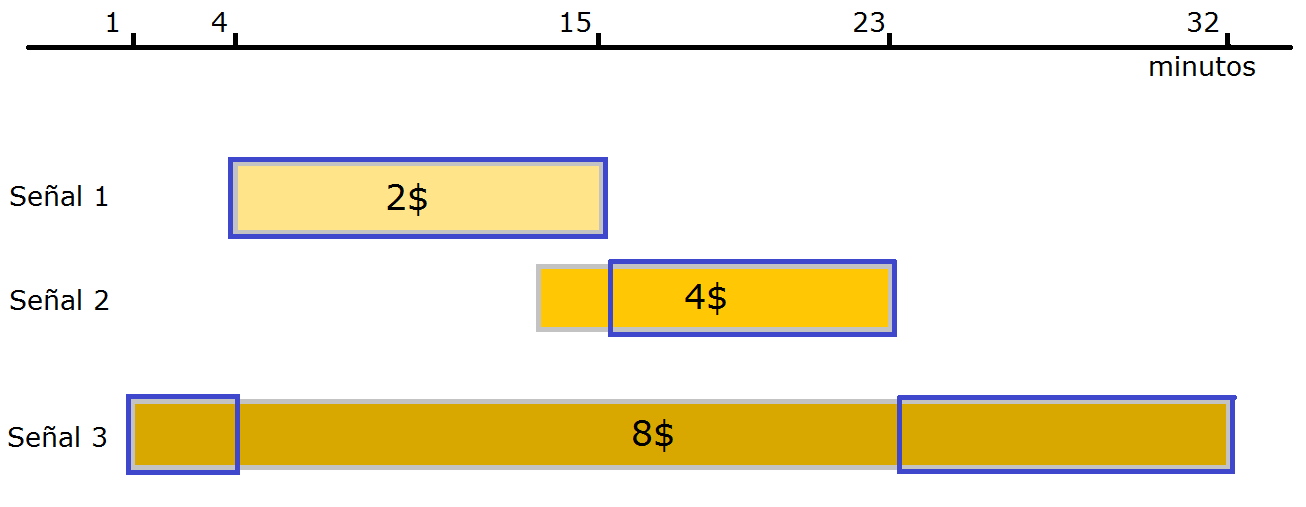
\includegraphics[scale=0.45]{imagenes/ej2/ejemplo1.png}
 	\caption{Ejemplo 1}
 	\label{ej1}	
   \end{center}
 \end{figure}

 \begin{figure}[h!]
   \begin{center}
 	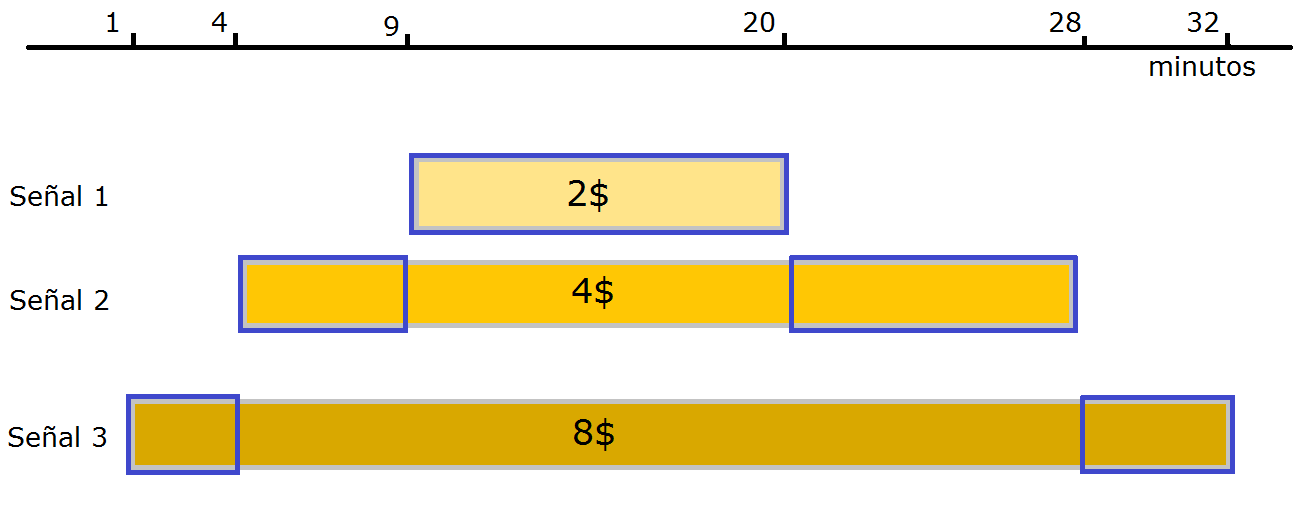
\includegraphics[scale=0.45]{imagenes/ej2/ejemplo2.png}
 	\caption{Ejemplo 2}
% 	\label{caballito}	
   \end{center}
 \end{figure}


\newpage

\subsection{Resoluci\'on propuesta y justificaci\'on}

El algoritmo que utilizamos pertenece a la familia de \emph{Divide \& Conquer}.\\

%\textcolor{red}{Aca pasa lo mismo de la implementacion porque hablamos mucho de vector y bla...}\\

El primer paso consiste en ordenar las frecuencias de menor a mayor en base al costo de cada una.\\

Luego, se sigue el esquema cl\'asico de Divide \& Conquer:\\

	\begin{codesnippet}
	\begin{verbatim}
divide(conjuntoDeFrecuencias F){
    Si hay mas de un elemento:
        Divido F en mitades A, B.
        intervalosA = divide(A)
        intervalosB = divide(B)
        Devuelvo conquer(intervalosA, intervalosB)
    Si hay un solo elemento:
        Lo devuelvo.	
}
	\end{verbatim}
	\end{codesnippet}

En palabras, si hay una sola frecuencia, la devolvemos, pues es trivial que su intervalo de duraci\'on es el m\'as barato y el de mayor extensi\'on temporal.\\

Si esto no ocurre, se seguirá subdividiendo hasta llegar al caso en el que hay solo un intervalo.
Es importante aclarar (pues es fundamental para el funcionamiento del algoritmo), que intervalosA tendrá la mitad de frecuencias más baratos, e intervalosB, la mitad de frecuencias más caros. Esto ocurre pues las frecuencias fueron ordenadas por su costo antes de comenzar con este tramo del algoritmo\\

Nuestro algoritmo de Merge (\emph{conquer}) se encarga de elegir entre las frecuencias de dos conjuntos pasados como parámetro, de modo que devuelve un sólo conjunto indicando los intervalos ocupados por las frecuencias elegidas (es decir, se toman la frecuencia más barata a cada momento, y se hacen los cortes pertinentes a cada frecuencia, según corresponda. \emph{Véase Fig:\ref{ej1} para saber c\'omo se recortan las frecuencias}).\\

Dado el enunciado del problema, para elegir qu\'e frecuencia utilizar en determinado intervalo de tiempo, se debe priorizar el costo m\'as barato emitiendo se\~nal siempre que sea posible.\\

Gracias a que en el primer llamado de nuestra funci\'on estas se encontraban en orden creciente respecto del precio, en cada paso del \emph{conquer} (sobre los dos conjuntos de entrada con intervalos) se van a priorizar los de la izquierda \textit{-intervalosA-}. Es decir que en cada paso, todos los intervalos pertenecientes a intervalosA (ya que son los de menor precio) van a pertencer al conjunto resultado. Mientras que s\'olo los intervalos que completen los tiempo sin se\~nal restantes pertenecientes al conjunto de la derecha \textit{-intervalosB-} van a ser colocados en el conjunto resultado (es decir, se completarán los vacíos entre frecuencias del primer conjunto, con frecuencias o intervalos de frecuencias de \'este conjunto). Esto representa un \emph{invariante} que se va a cumplir en cada paso del algoritmo, lo cual nos permite justificar que la soluci\'on obtenida es la deseada.\\

%	\begin{codesnippet}
%	\begin{verbatim}
%conquer(conjuntoDeFrecuencias A, conjuntoDeFrecuencias B){
%	vector<frecuencia>::iterator iterCara = cara.begin(), iterBarata = barata.begin();
%	vector<frecuencia> res;
%	
%	En el conjunto res voy a tener el resultado.
%    Voy recorriendo en orden A y B, mientras haya elementos en A:
%    //Llamo A[i] al intervalo actual de A y B[j] al de B.
%        Si B[j] comienza antes que A[i]:
%            Si B[j] termina antes que A[i]:
%                Inserto B[j] en res.
%                j++
%            Si B[j] termina despues que A[i] empiece                                                                                                                                                                                                                                                                                                                                                                                                                                                                                                                                                                                                                                                                                                                                                                                                                                                                                                                                                                                                                                                                                                                                                                                                                                                                                                                                                              :
%                
%    
%    
%        Si A[i] comienza antes que B[j]:
%            Inserto A[i] en res
%            Si B[j] se superpone en algun momento con A[i]:
%                Al comienzo de B[j] le asigno el final de A[i]
%
%
%
%
%	while(iterCara != cara.end()){
%		if(iterBarata != barata.end()){
%			if(iterCara->principio < iterBarata->principio){ //la cara empieza antes
%				if(iterCara->fin <= iterBarata->principio){ //la cara termina antes de que empiece la barata
%					res.push_back(*iterCara);				//meto la cara entera
%					iterCara++;
%				}
%				else{ //la cara empieza antes y termina despues del principio de la barata
%					frecuencia antes;
%					antes.id = iterCara->id;
%					antes.costo = iterCara->costo;
%					antes.principio = iterCara->principio;
%					antes.fin = iterBarata->principio;
%					res.push_back(antes);
%					iterCara->principio = iterBarata->fin;
%				}
%			}
%			else{ //la barata empieza antes (o igual) que la cara
%				if(iterCara->fin > iterBarata->fin){ //la cara termina despues que la barata
%					if (iterCara->principio < iterBarata->fin) //este if es nuevo
%						iterCara->principio = iterBarata->fin;
%					res.push_back(*iterBarata);
%					iterBarata++;
%				}
%				else
%					iterCara++;
%			}
%		}
%		else{
%			if(iterCara->principio < iterCara->fin)
%				res.push_back(*iterCara);
%			iterCara++;
%		}
%	}
%	while(iterBarata != barata.end()){
%		res.push_back(*iterBarata);
%		iterBarata++;
%	}
%	return res;
%}
%
%	\end{verbatim}
%	\end{codesnippet}

Este \'ultimo paso hace uso exhaustivo del invariante: todos los intervalos del conjunto intervalosA deben pertenecer al conjunto soluci\'on, y lo \'unico que se debe agregar son los intervalos de intervalosB que o bien aumentan el rango de tiempo para transmitir (uso el servicio desde antes o m\'as tiempo) o bien completan gaps que puedan existir entre las frecuencias m\'as baratas.

%Este algoritmo resuelve lo propuesto dando una soluci\'on \'optima porque del modo en que est\'a definido, primero divide al grupo con todas las frecuencias ofrecidas recursivamente hasta llegar a conjuntos con una sola frecuencia. Luego, al momento de mergear estos grupos de a dos, siempre prioriza al grupo de la izquierda (el m\'as barato). 

%Esto quiere decir que en el primer paso de este \textit{merge} se van a comparar solamente dos frecuencias entre s\'i, colocando la frecuencia m\'as barata completa y; si la oferta de intervalos de la frecuencia m\'as cara completa uno o dos intervalos donde no se le hab\'ia asignado se\~nal, se le otorga a ellos la frecuencia m\'as cara. De este modo, comparamos de a dos, frecuencias consecutivas otorg\'andole prioridad a la frecuencia m\'as barata. \textcolor{red}{Poner dibujito.} 

%En el siguiente paso del \textit{merge} se van a comparar dos conjuntos de intervalos con dos frecuencias en cada uno. Cada uno de estos conjuntos puede estar conformado por uno, dos o tres intervalos. \textcolor{red}{Poner dibujito} Gracias al formato de nuestro algoritmo, en cada paso del merge se preserva el invariante de que el conjunto ubicado a la izquierda tiene las frecuencias m\'as baratas mientras que el de la derecha tiene las m\'as caras. Se prosigue de manera an\'aloga a lo anterior, se preservan todos los intervalos de frecuencias pertenecientes al conjunto de los m\'as baratos y s\'olo se agregan frecuencias del conjunto caro en caso de que esten disponibles en intervalos de tiempos que hayan quedado vac\'ios.

%Estos pasos se van a reiterar, comparando conjuntos de intervalos entre dos, hasta que se hayan recorrido todas las frecuencias.\\

%Una vez terminados todos los pasos recursivos, vamos a contar con el conjunto de intervalos que completen la mayor cantidad de tiempo con el costo m\'as bajo. Si no hay dos frecuencias con el mismo costo, esta soluci\'on (\'optima) es \'unica, en caso contrario podr\'ia existir m\'as de una soluci\'on \'optima. \\

\newpage

\subsection{An\'alisis de la complejidad}

La primera ejecuci\'on que realiza el algoritmo es ordenar a las frecuencias de menor a mayor (dado que definimos el operador $<$ tal que: $frecA<frecB$ $\Rightarrow$ $costo(frecA)<costo(frecB)$). Este ordenamiento lo realizamos mediante el algoritmo \href{http://www.cplusplus.com/reference/algorithm/sort/}{sort()} \footnote{http://www.cplusplus.com/reference/algorithm/sort/}, el cual cuenta con una complejidad de $O(n.log(n))$.\\
\\

Para realizar el análisis de la ejecuci\'on siguiente del algoritmo, es necesario calcular cu\'antos intervalos contendr\'a, como m\'aximo, el conjunto soluci\'on (desde ahora ``\emph{CS}''). Este valor ser\'a $2n-1$, siendo $n$ la cantidad de frecuencias dadas como par\'ametro.

Esto se deduce de analizar las posibles entradas para el algoritmo. Primero vamos a analizar el caso donde no existan dos frecuencias pasadas como par\'ametro con el mismo valor. De este modo la soluci\'on \'optima al problema va a ser \'unica. \\


Supongamos \textbf{n=1}. El intervalo de la frecuencia pasada como par\'ametro ser\'a el \'unico elemento del \emph{CS} y verifica $2n-1$ $=$ $2$.$1-1$ $=$ $1$.\\

Luego, tomamos \textbf{n=2}. De este modo, ambas pueden solaparse o ser disjuntas. Llamamos $1$ a la frecuencia m\'as barata y $2$ a la m\'as cara, $1$ va a estar incluida completa en \emph{CS} y $2$ puede formar dos intervalos, uno o ninguno. A continuaci\'on, se adjuntan cada uno de los casos, indicando en naranja los intervalos que pertenecer\'an a \emph{CS}.\\

La frecuencia $2$ no forma ning\'un intervalo:

 \begin{figure}[h!]
   \begin{center}
 	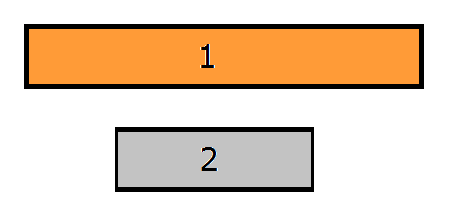
\includegraphics[scale=0.45]{imagenes/ej2/secuencias/Paso1/Caso0.png}
% 	\caption{}
% 	\label{caballito}	
   \end{center}
 \end{figure}

La frecuencia $2$ forma un intervalo:

 \begin{figure}[h!]
   \begin{center}
 	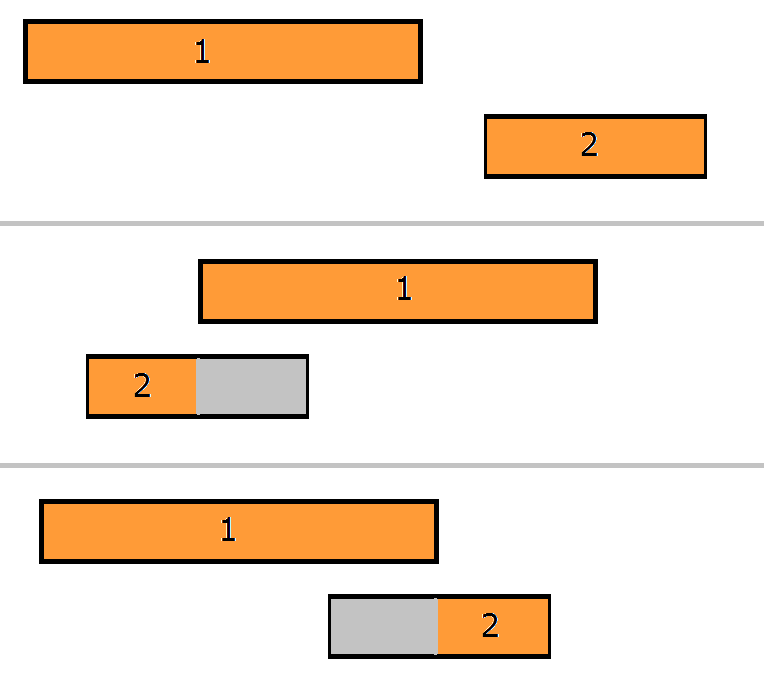
\includegraphics[scale=0.45]{imagenes/ej2/secuencias/Paso1/Caso1.png}
% 	\caption{}
% 	\label{caballito}	
   \end{center}
 \end{figure}
 

 \newpage
La frecuencia $2$ forma dos intervalos: 
 
  \begin{figure}[h!]
   \begin{center}
 	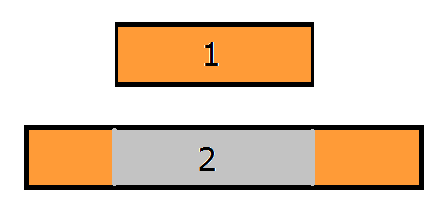
\includegraphics[scale=0.45]{imagenes/ej2/secuencias/Paso1/Caso2.png}
% 	\caption{}
% 	\label{caballito}	
   \end{center}
 \end{figure}
 


Es decir, para n=2 la cantidad m\'axima de intervalos posibles es $3$ intervalos, lo cual tambi\'en cumple $2n-1$ $=$ $2$.$2-1$ $=$ $3$.\\
 
%, entonces dado una frecuencia (la m\'as barata), la otra (m\'as cara) puede que se solape o no. Si no lo hace, entonces el CS tendr\'a ambos intervalos incluidos. Si se solapa, 1) est\'a inclu \'ido, con lo cual el CS ser\'a contendr\'a solo a la primer frecuencia; 2) arranca o termina mientras la otra est\'a disponible, dejando al CS con \'unicamente el pedazo de intervalo que no se solapa y el otro entero; o bien 3) arranca y termina antes y despu\'es de que arranque y termina el primero, logrando que el CS tenga un primer intervalo de la segunda frecuencia, hasta que arranca la primera, que entra por completo y luego un segundo intervalo de la segunda frecuencia que empieza cuando termina la primera. Esto se extiende para todo n con los mismos resultados, solo que puede agregarse un 4) completar un gap.\\

Al momento de tomar \textbf{n=3}, lo hacemos considerando las frecuencias $1$, $2$ y $3$. Partimos del caso anterior al que le a\~nadimos la frecuencia $3$. Es decir, vamos a contar con a lo sumo $3$ intervalos. La distribuci\'on de los intervalos se va a dar de la siguiente manera:\\

  \begin{figure}[h!]
   \begin{center}
 	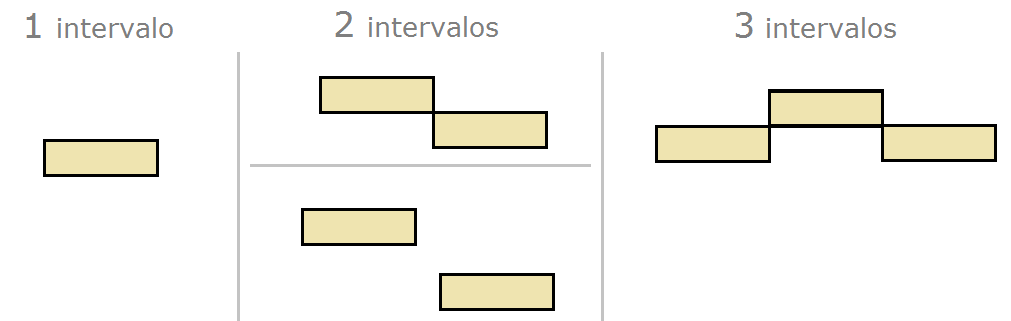
\includegraphics[scale=0.45]{imagenes/ej2/secuencias/salida2.png}
% 	\caption{}
% 	\label{caballito}	
   \end{center}
 \end{figure}

Podemos observar que de las cuatro distribuciones distintas que pueden ocurrir, en s\'olo una los intervalos son completamente disjuntos, esto es en el caso donde se a\~nadi\'o el intervalo $2$ completo. En los dem\'as casos, si bien pueden ser uno, dos o tres intervalos distintos al unirlos conforman un intervalo continuo, por lo cual entre ellos no va a haber gaps, es decir s\'olo se podr\'an a\~nadir intervalos en los bordes. Por este motivo, a estos casos los tomamos an\'alogos al caso de $n=2$ donde se agregar\'an a lo sumo dos intervalos, lo cual conforma en el caso m\'aximo 3 intervalos pre-existentes y 2 nuevos, dando un total de 5. Esto cumple lo planteado $2n-1$ $=$ $2$.$3-1$ $=$ $5$.\\

Ahora debemos considerar por separado, el caso donde contamos con dos intervalos pre-existentes totalmente disjuntos.\\

El \'unico caso donde se adicionan tres intervalos es el siguiente:\\
  \begin{figure}[h!]
   \begin{center}
 	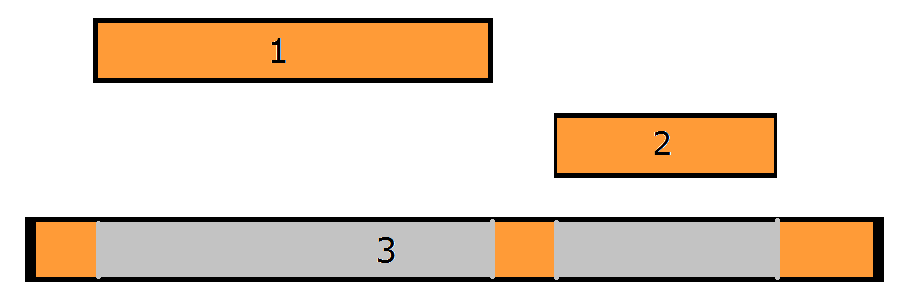
\includegraphics[scale=0.45]{imagenes/ej2/secuencias/Paso2/Caso3.png}
% 	\caption{}
% 	\label{caballito}	
   \end{center}
 \end{figure}
\newpage

Los casos donde se adicionan dos intervalos son los mostrados a continuaci\'on:
  \begin{figure}[h!]
   \begin{center}
 	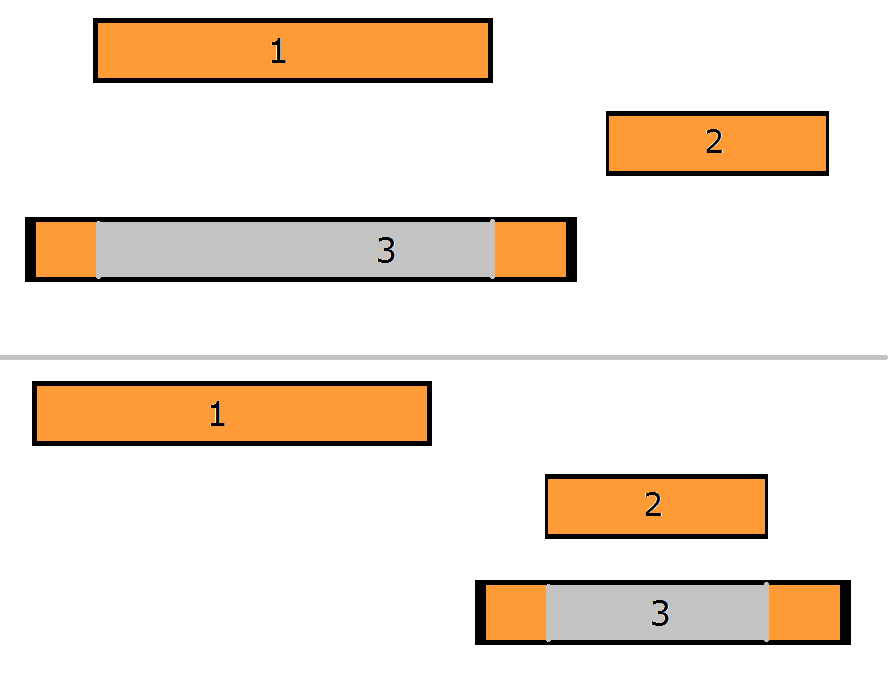
\includegraphics[scale=0.45]{imagenes/ej2/secuencias/Paso2/todos2.png}
% 	\caption{}
% 	\label{caballito}	
   \end{center}
 \end{figure}


Los siguientes son los casos donde al agregar la frecuencia $3$ s\'olo se adiciona un intervalo:
  \begin{figure}[h!]
   \begin{center}
 	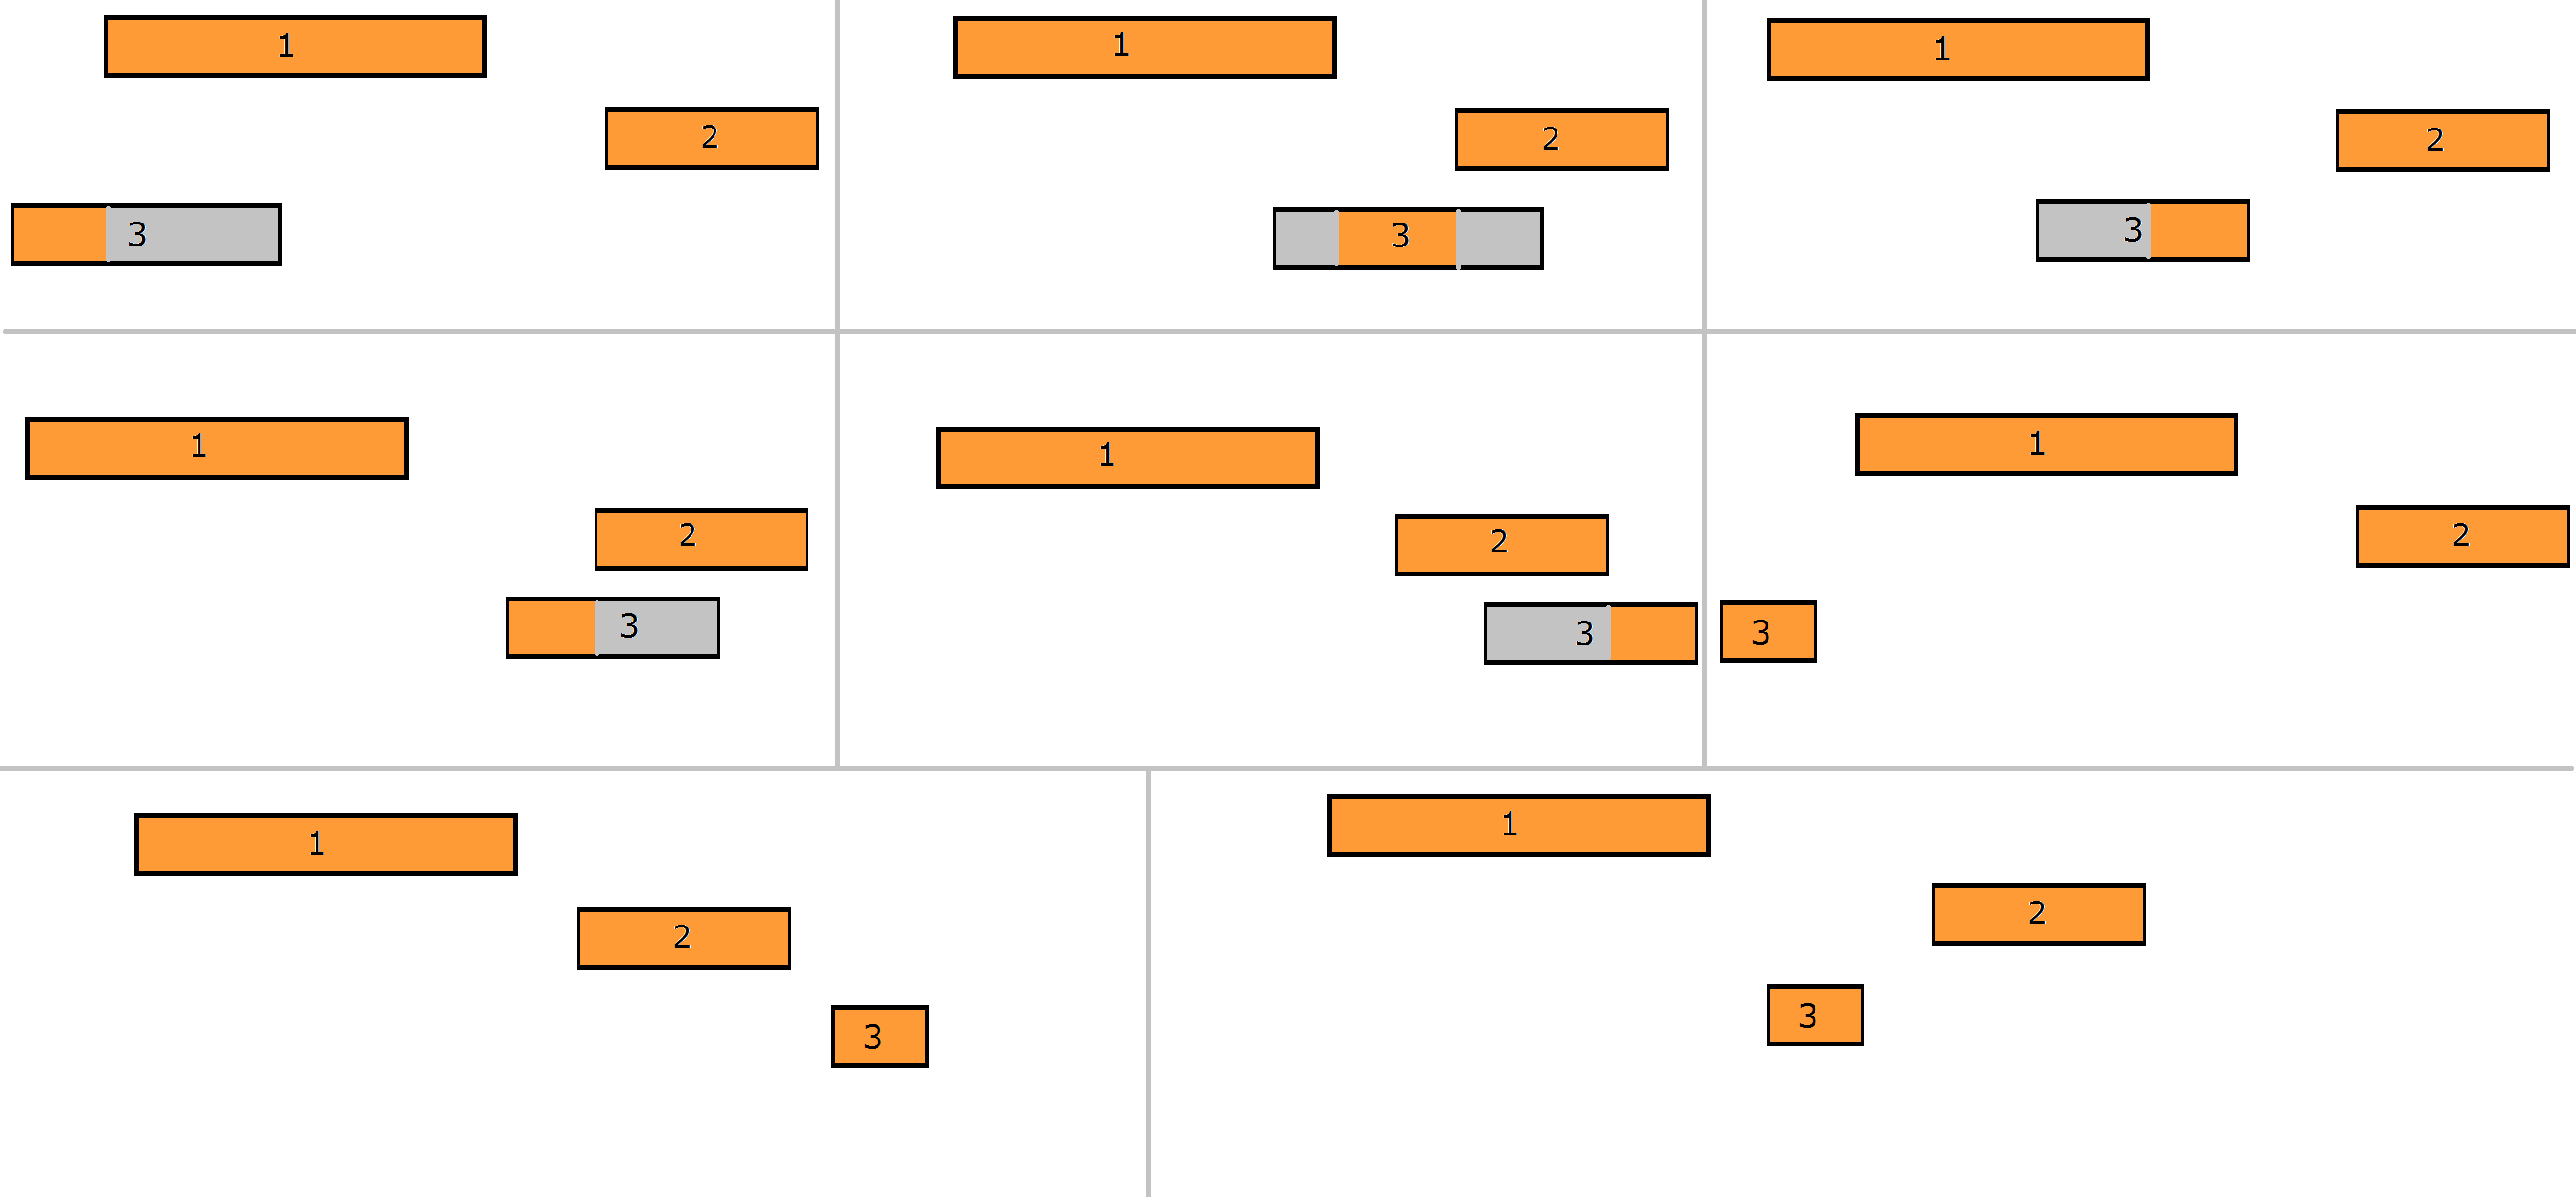
\includegraphics[scale=0.2]{imagenes/ej2/secuencias/Paso2/todos1.png}
% 	\caption{}
% 	\label{caballito}	
   \end{center}
 \end{figure}

Por consiguiente, el m\'aximo de intervalos que pueden a\~nadirse son tres, considerando siempre s\'olo dos pre-existentes, lo cual da un total de 5 que cumple: $2n-1$ $=$ $2$.$3-1$ $=$ $5$.\\

%Hasta el caso 3) se ve claramente que el m\'aximo n\'umero de intervalos es el propuesto (agregar un intervalo a izquierda y uno a derecha). Para el caso 4) hay que tener en cuenta que el paso anterior fue un caso de no solapamiento, es decir que si intercambiara la frecuencia que completa gaps con la no solapada, entonces entrar\'ia en el caso 2) o en el caso 3), verificando que a lo sumo se llega a \emph{2n-1} intervalos.\\

Si extendemos este c\'alculo para cualquier n, vamos a concluir que siempre la cantidad de intervalos va a estar acotada por $2n-1$ ya que se puede reducir el problema a cualquiera de las situaciones mencionadas.\\%\textcolor{red}{Habra que explicar un poco mas? O con esto basta?}


Partimos de la hip\'otesis de que los costos de las frecuencias eran todos distintos, lo cual nos asegura una soluci\'on \'unica con una cantidad \'unica de intervalos. Ahora, si consideramos que pueden existir dos (o m\'as) frecuencias, llamemos \emph{A} y \emph{B}, con el mismo precio podemos asumir indistintamente que \emph{A$<$B} o \emph{A$>$B} lo cual podr\'ia devolver intervalos distintos, pero siempre su cantidad va a estar acotada por lo mismo probado anteriormente: $2n-1$.\\

\newpage

Una vez que ya acotamos la cantidad final de intervalos por $2n-1$, podemos proceder al an\'alisis de complejidad del algoritmo de Divide \& Conquer.\\

El algoritmo \emph{divide} particiona el problema en dos subproblemas m\'as chicos, en particular de la mitad de tamaño que el problema original, lo que implica que tiene complejidad \emph{T(n)=2T(n/2)+O(conquer)} (ecuación que surge de llamar recursivamente a la función \emph{divide}).\\

La funci\'on \emph{conquer} va a recorrer, en el peor caso, dos vectores cuyas longitudes son $(2n-1)/2$ para cada uno y va a aplicar operaciones que toman $O(1)$ para cada una de ellos. El vector que va construyendo con el CS toma $O(2n-1)$ que es igual a $O(n)$.

 Estas complejidades se suman y por propiedades de $O$ se obtiene que $O(conquer)$ resulta $O(n)$.\\

Reemplazando en la ecuaci\'on obtenemos: \emph{T(n)=2T(n/2)+O(n)}. Vemos que es la misma ecuaci\'on de recurrencia que el algortimo de MergeSort, que por \emph{Teorema Maestro} se deduce que tiene complejidad $O(n.log(n))$.\\
\\

Dado que cont\'abamos con una complejidad inicial de $O(n.log(n))$, la complejidad resultante del algoritmo es $O(n.log(n))+O(n.log(n))$ que equivale a una complejidad de $O(n.log(n))$, como prentend\'iamos.

\newpage
\subsection{C\'odigo fuente}



	\begin{codesnippet}
	\begin{verbatim}
struct frecuencia{
    long int id;
    long int costo;
    long int principio;
    long int fin;
    bool operator< (const frecuencia& otro) const{
        if(costo == otro.costo){
            if(principio == otro.principio)
                return fin > otro.fin;
            return principio < otro.principio;
        }
        return costo < otro.costo;
    }
};
	\end{verbatim}
	\end{codesnippet}
	
		\begin{codesnippet}
	\begin{verbatim}
int main(int argc, char const *argv[]){
    chrono::time_point<chrono::system_clock> start, end;
    long int cantFrec;
    vector<frecuencia> frecuencias;
    //Leemos informacion del problema
    cin >> cantFrec;
    for (int i = 0; i < cantFrec; ++i){
        frecuencia actual;
        actual.id = i;
        cin >> actual.costo;
        cin >> actual.principio;
        cin >> actual.fin;
        if(actual.fin > actual.principio)
        frecuencias.push_back(actual);
    }
    start = chrono::system_clock::now();
    //Aplicamos el algoritmo
    vector<frecuencia> optimas = altaFrecuencia(frecuencias);
    vector<frecuencia>::iterator iter;
    //Calculamos el costo total (lo tuvimos en cuenta en la medicion de tiempos y complejidad)
    long int costoTotal = 0;
    for (iter = optimas.begin(); iter != optimas.end(); iter++){
        costoTotal += (iter->fin - iter->principio) * iter->costo;
    }
    end = chrono::system_clock::now();
    //Stdout pedido
    cout << costoTotal << endl;
    for (iter = optimas.begin(); iter != optimas.end(); iter++){
        cout << iter->principio << " " << iter->fin << " " << iter->id + 1 << endl;
    }
    cout << "-1" << endl;
    chrono::duration<double> elapsed_seconds = end-start;
    cout << "Tiempo: " << elapsed_seconds.count() << endl;
    return 0;
}
	\end{verbatim}
	\end{codesnippet}
	
	
		\begin{codesnippet}
	\begin{verbatim}
vector<frecuencia> altaFrecuencia(vector<frecuencia>& frecuencias){
    //Ordenamos el vector de menor a mayor costo de cada frecuencia
    sort(frecuencias.begin(), frecuencias.end());
    return divide(frecuencias, 0, frecuencias.size()-1);
}
	\end{verbatim}
	\end{codesnippet}

	
		\begin{codesnippet}
	\begin{verbatim}
vector<frecuencia> divide(vector<frecuencia>& frecuencias, long int comienzo, long int final){
    //Si tenemos dos o mas frecuencias, llamos a divide con cada una las mitades
    // y luego combinamos las soluciones
    if(final - comienzo > 0){
        vector<frecuencia> barata = divide(frecuencias, comienzo, (final+comienzo)/2);
        vector<frecuencia> cara = divide(frecuencias, ((final+comienzo)/2)+1, final);
        return conquer(barata, cara);
    }
    //Si solo hay una frecuencia,esta sera la forma mas barata y de maximo tiempo para transmitir
    else{
        vector<frecuencia> res;
        res.push_back(frecuencias[comienzo]);
        return res;
    }
}
	\end{verbatim}
	\end{codesnippet}
	
	
		\begin{codesnippet}
	\begin{verbatim}
vector<frecuencia> conquer(vector<frecuencia> barata, vector<frecuencia> cara){
    vector<frecuencia>::iterator iterCara = cara.begin(), iterBarata = barata.begin();
    vector<frecuencia> res;
    //mientras tenga frecuencias caras
    while(iterCara != cara.end()){
        // si todavia tengo baratas
        if(iterBarata != barata.end()){
            // si la cara empieza antes que la barata
            if(iterCara->principio < iterBarata->principio){
                // si la cara termina antes de que empiece la barata o al mismo tiempo
                if(iterCara->fin <= iterBarata->principio){
                    // la cara es parte de la solucion
                    res.push_back(*iterCara);
                    iterCara++;
                }
                // sino la cara empieza antes y termina despues del principio de la barata
                else{
                    // agrego el pedazo de cara que es solucion 
                    // y le digo que su nuevo principio es el fin de la barata
                    frecuencia antes;
                    antes.id = iterCara->id;
                    antes.costo = iterCara->costo;
                    antes.principio = iterCara->principio;
                    antes.fin = iterBarata->principio;
                    res.push_back(antes);
                    iterCara->principio = iterBarata->fin;
                }
            }
            // sino la barata empieza antes o al mismo tiempo que la cara
            else{
                // si la cara termina despues que la barata
                if(iterCara->fin > iterBarata->fin){
                    // si la cara intersecta con la barata, 
                    //le digo que su nuevo principio es el fin de la barata
                    if (iterCara->principio < iterBarata->fin)
                    iterCara->principio = iterBarata->fin;
                    // la barata es parte de la solucion
                    res.push_back(*iterBarata);
                    iterBarata++;
                }
                // si no salteo la cara, hay una o mas frecuencias para el tiempo 
                //en que se puede utilizar que son mas baratas
                else
                iterCara++;
            }
        }
        // sino agrego todas las caras restantes a la solucion
        else{
            if(iterCara->principio < iterCara->fin)
            res.push_back(*iterCara);
            iterCara++;
        }
    }
    //si me quede sin caras, agrego las baratas restantes a la solucion
    while(iterBarata != barata.end()){
        res.push_back(*iterBarata);
        iterBarata++;
    }
    return res;
}
	\end{verbatim}
	\end{codesnippet}
		
	
\newpage
\subsection{Experimentaci\'on}

\subsubsection{Constrastaci\'on Emp\'irica de la complejidad}

Para llevar a cabo la experimentaci\'on, consideramos distintos sets de frecuencias con sus intervalos y costos generados aleatoriamente. Cada uno de ellos var\'ia en tama\~no.\\

Los tiempos de ejecuci\'on para cada tama\~no distinto de n (cantidad de frecuencias) fueron los siguientes:


\begin{table}[htb]
\centering
\begin{tabular}[c]{|l|l|}

		\hline
n & Tiempo en segundos\\
		\hline
100	&	0.000415645\\
		\hline
150	&	0.00049622\\
		\hline
200	&	0.000595058\\
		\hline
300	&	0.000752836\\
		\hline
400	&	0.001029706\\
		\hline
500	&	0.001253788\\
		\hline
750	&	0.001757269\\
		\hline
1000	&	0.0023792\\
		\hline
1500	&	0.003352018\\
		\hline
2000	&	0.004313126\\
		\hline
3000	&	0.006464969\\
		\hline
5000	&	0.010964701\\
		\hline
6500	&	0.013377069\\
		\hline
8000	&	0.01643833\\
		\hline
9500	&	0.0197472\\
		\hline
10500	&	0.021750165\\
		\hline
11500	&	0.024404865\\
		\hline
12500	&	0.02591816\\
		\hline
		
		
		
	\end{tabular}
%\caption{Tabla muy sencilla.}
%\label{tabla:sencilla2}
\end{table}


  \begin{figure}[h!]
   \begin{center}
 	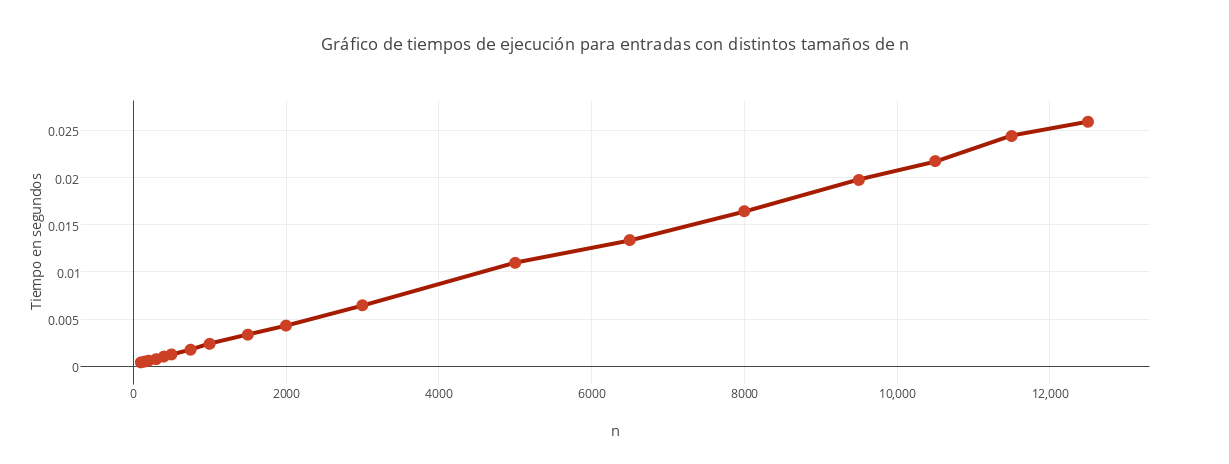
\includegraphics[scale=1.7]{imagenes/ej2/grafiquitos/graf1.png}
% 	\caption{}
% 	\label{caballito}	
   \end{center}
 \end{figure}
 \newpage
%   \begin{figure}[h!]
%   \begin{center}
% 	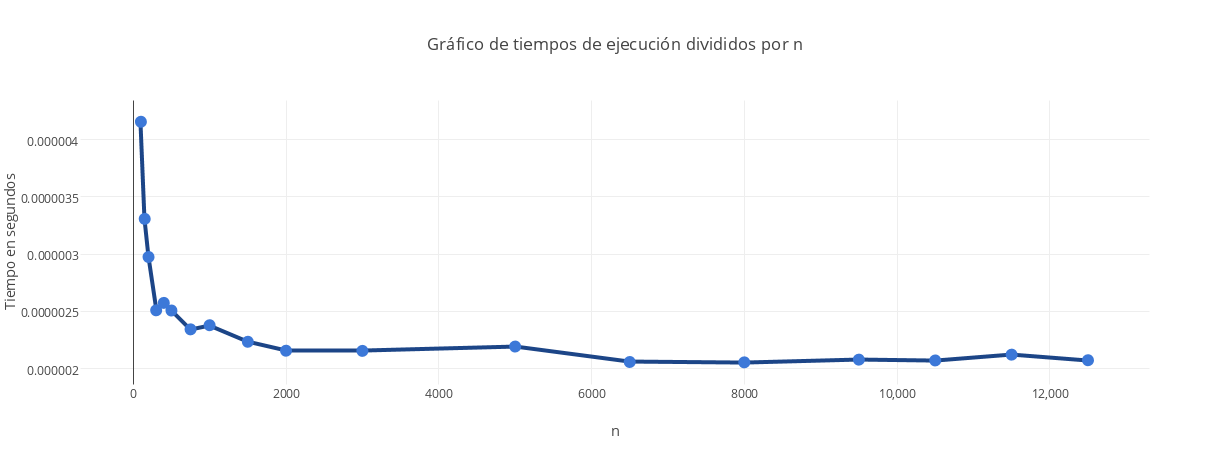
\includegraphics[scale=1.7]{imagenes/ej2/grafiquitos/graf2.png}
% 	\caption{}
% 	\label{caballito}	
%   \end{center}
% \end{figure}

Dado que la Cota de Complejidad planteada te\'oricamente es de $O(n.log(n))$, era esperable que la curva sea creciente (ya que $f(n)=k.n.log(n)+q$ -considerando a $k$ y $q$ constantes- lo es). 

A simple vista, no se puede apreciar si la relaci\'on que tienen respecto de tama\~no/tiempo es la caracter\'istica de $f(n)$. Por este motivo, como siguiente paso decidimos linealizar los tiempos, dividiendo a cada uno por $log(n)$.


\begin{table}[htb]
\centering
\begin{tabular}[c]{|l|l|}

		\hline
n & Tiempo en segundos dividido por log$_2$(n)\\ 
 	\hline
100	&	0.000207823	\\
 	\hline
 150	&	0.000228033	\\
	\hline
 200	&	0.000258605	\\
	\hline
 300	&	0.000303916	\\
	\hline
 400	&	0.000395727	\\
	\hline
 500	&	0.000464543	\\
	\hline
 750	&	0.000611211	\\
	\hline
 1000	&	0.000793067	\\
	\hline
 1500	&	0.001055391	\\
	\hline
 2000	&	0.0013066	\\
	\hline
 3000	&	0.001859288	\\
	\hline
 5000	&	0.002964258	\\
	\hline
 6500	&	0.003508359	\\
	\hline
 8000	&	0.00421162	\\
	\hline
 9500	&	0.004964447	\\
	\hline
 10500	&	0.005408889	\\
	\hline
 11500	&	0.006010017	\\
	\hline
 12500	&	0.00632627	\\
	\hline
  	
		
		
		
	\end{tabular}
%\caption{Tabla muy sencilla.}
%\label{tabla:sencilla2}
\end{table}
 
   \begin{figure}[h!]
   \begin{center}
 	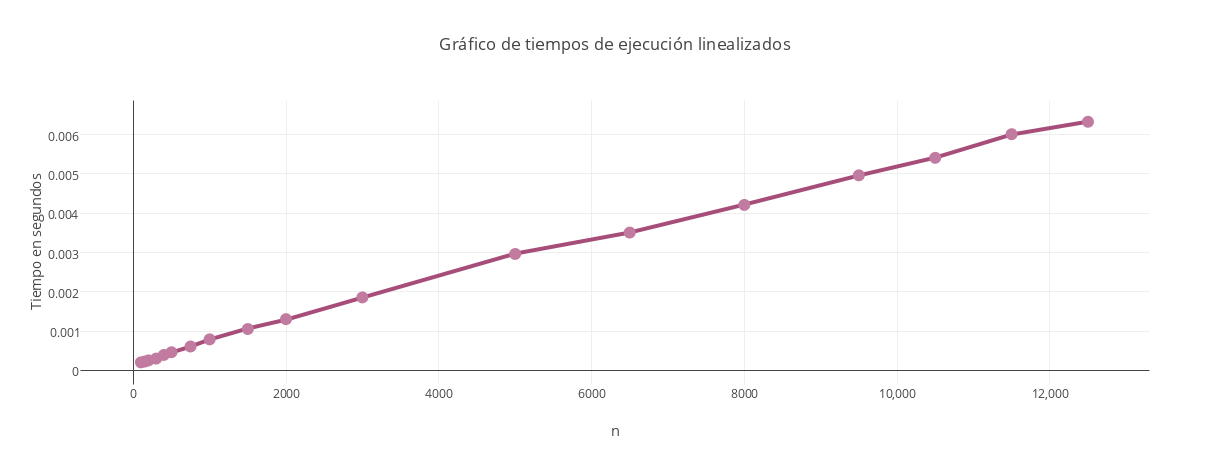
\includegraphics[scale=1.7]{imagenes/ej2/grafiquitos/graf3.png}
% 	\caption{}
% 	\label{caballito}	
   \end{center}
 \end{figure}
 
 
 Si bien la morfolog\'ia del segundo gr\'afico parece similar a la anterior, en este caso la funci\'on que est\'abamos buscando era $g(n)=kn+q$ (siendo $k$ y $q$ alguna constante). Acorde a lo perceptible al ojo humano, la curva graficada se condice con alguna recta.\\
 
 De este modo, deducimos que nuestra experimentaci\'on condice a la Cota Te\'orica planteada de $O(n.log(n))$.